\definecolor{ovA}{RGB}{36,92,160}
\definecolor{ovB}{RGB}{196,86,18}
\definecolor{ovC}{RGB}{28,122,74}
\begin{tikzpicture}[
  font=\sffamily\scriptsize,
  >={Stealth[length=2.2mm]},
  spr/.style={inner sep=0.4pt, draw=black!25, line width=0.35pt, fill=white},
  box/.style={draw=#1!75!black, fill=#1!12, rounded corners=2pt, align=center,
              inner sep=2.4pt, line width=0.65pt, font=\sffamily\scriptsize},
  note/.style={align=center, font=\sffamily\tiny, text=black!62},
  arr/.style={->, line width=0.85pt, draw=#1!80!black},
]
\def\S{1.18cm}
\newcommand{\badge}[2]{%
  \tikz[baseline=-0.6ex]\node[circle, fill=white, text=#1, font=\sffamily\bfseries\scriptsize,
    inner sep=0.9pt, minimum size=0.32cm]{#2};}
\newcommand{\panel}[6]{% x0 y0 x1 y1 colour title
  \fill[#5!7, rounded corners=3.5pt] (#1,#2) rectangle (#3,#4);
  \draw[#5!55, rounded corners=3.5pt, line width=0.7pt] (#1,#2) rectangle (#3,#4);
  \fill[#5, rounded corners=3.5pt] (#1,#4-0.42) rectangle (#3,#4);
  \fill[#5] (#1,#4-0.42) rectangle (#3,#4-0.18);
  \node[anchor=west, text=white, font=\sffamily\bfseries\scriptsize] at (#1+0.10,#4-0.21) {#6};}

% ── 1 ────────────────────────────────────────────────────────────────
\panel{0.00}{0.00}{7.55}{3.55}{ovA}{\badge{ovA}{1}\;Native-Resolution Target Rebuilding}
\node[spr] (d1) at (0.92,2.15) {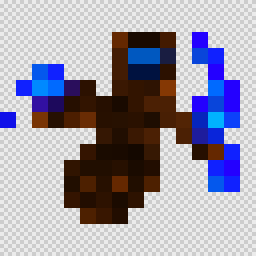
\includegraphics[width=\S]{figures/ov/down.png}};
\node[spr] (d2) at (0.92,0.85) {
\includegraphics[width=\S]{figures/ov/down2.png}};
\node[note, text=ovA!50!black] at (0.92,2.88) {49 colours};
\node[note, rotate=90, text=ovA!45!black] at (0.16,1.50) {downscaled targets};

\node[box=ovA, text width=2.38cm, anchor=west] (c1) at (1.82,2.55)
  {\textbf{dedup} --- no train/test leakage};
\node[box=ovA, text width=2.38cm, anchor=west] (c2) at (1.82,1.55)
  {\textbf{bucket} --- shrink at most $1.5\times$};
\node[box=ovA, text width=2.38cm, anchor=west] (c3) at (1.82,0.55)
  {\textbf{+15k} licensed sprites, 40\% native $\le$24\,px};
\draw[ovA!65, line width=0.7pt] (1.82,0.55) -- (1.82,2.55);
\draw[arr=ovA] (1.55,1.50) -- (1.80,1.50);
\draw[arr=ovA] (4.28,1.50) -- (4.55,1.50);

\node[spr] (n1) at (5.22,2.15) {
\includegraphics[width=\S]{figures/ov/native.png}};
\node[spr] (n2) at (5.22,0.85) {
\includegraphics[width=\S]{figures/ov/native2.png}};
\node[note, text=ovA!50!black] at (5.22,2.88) {6 colours, native};
\node[box=ovA, text width=1.55cm, font=\sffamily\tiny] at (6.72,1.50)
  {\textbf{native protocol}\\[1pt] FD vs.\ sprites drawn at $\le R$\,px};

% ── 3 ────────────────────────────────────────────────────────────────
\panel{7.70}{0.00}{13.95}{3.55}{ovC}{\badge{ovC}{3}\;Palette Refinement}
\node[spr] at (8.45,2.15) {
\includegraphics[width=\S]{figures/ov/ext.png}};
\node[spr] at (8.45,0.85) {
\includegraphics[width=\S]{figures/ov/ext2.png}};
\node[note] at (8.45,2.88) {external sprite};
\node[box=ovC, text width=1.22cm] (rn) at (10.00,1.50) {\textbf{re-noise}\\to $\sigma$\\[-1pt]{\tiny SDEdit}};
\node[box=ovB, text width=1.22cm] (dn) at (11.50,1.50) {\textbf{denoise}\\with PPS\\[-1pt]{\tiny panel 2}};
\node[spr] at (13.10,2.15) {
\includegraphics[width=\S]{figures/ov/refined.png}};
\node[spr] at (13.10,0.85) {
\includegraphics[width=\S]{figures/ov/refined2.png}};
\node[note] at (13.10,2.88) {refined sprite};
\draw[arr=ovC] (9.10,1.50) -- (rn.west);
\draw[arr=ovC] (rn.east) -- (dn.west);
\draw[arr=ovC] (dn.east) -- (12.48,1.50);
\node[note, text=ovC!55!black] at (10.75,0.42) {$\sigma$ keeps layout, PPS repaints the medium};

% ── 2 ────────────────────────────────────────────────────────────────
\panel{0.00}{-3.55}{13.95}{-0.12}{ovB}{\badge{ovB}{2}\;Palette-Projected Sampling (PPS)}
\node[anchor=east, text=white, font=\sffamily\tiny] at (13.82,-0.33)
  {training-free $\cdot$ no extra NFEs $\cdot$ UNet or transformer};

\def\y{-1.85}
\node[spr] (xt) at (0.85,\y) {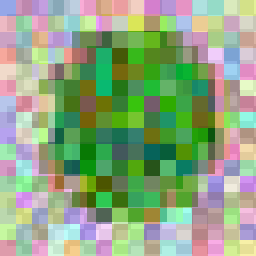
\includegraphics[width=\S]{figures/ov/xt.png}};
\node[note] at (0.85,\y+0.78) {noisy $x_t$};

\node[box=ovB, text width=1.85cm, minimum height=1.05cm] (un) at (2.95,\y)
  {\textbf{denoiser}\\$\epsilon_\theta(x_t,t,c,b)$\\[-1pt]{\tiny + ICG}};
\draw[arr=ovB] (xt.east) -- (un.west);

\node[spr] (x0) at (5.05,\y) {
\includegraphics[width=\S]{figures/ov/dither.png}};
\node[note] at (5.05,\y-0.88) {$\hat x_0$: $\sim$50 colours, dither};
\draw[arr=ovB] (un.east) -- (x0.west);

\node[box=ovB, fill=ovB!28, text width=2.05cm, minimum height=1.05cm] (pi) at (7.20,\y)
  {\textbf{project} $\Pi_k(\hat x_0)$\\per-sprite $k$-means\\on opaque pixels};
\draw[arr=ovB] (x0.east) -- (pi.west);

\node[spr] (xp) at (9.35,\y) {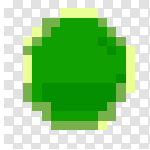
\includegraphics[width=\S]{figures/ov/pal.png}};
\node[note] at (9.35,\y-0.88) {$\hat x_0^{\mathrm{pal}}$: $k$ flat colours};
\draw[arr=ovB] (pi.east) -- (xp.west);

\node[box=ovB, text width=1.55cm, minimum height=1.05cm] (ep) at (11.35,\y)
  {\textbf{re-derive} $\tilde\epsilon$\\Eq.~(\ref{eq:palette})\\and step};
\draw[arr=ovB] (xp.east) -- (ep.west);

\node[spr] (out) at (13.15,\y) {
\includegraphics[width=\S]{figures/ov/pal2.png}};
\node[note] at (13.15,\y+0.78) {final sprite};
\draw[arr=ovB] (ep.east) -- (out.west);

\draw[arr=ovB, dashed, rounded corners=3pt]
  (ep.south) -- (11.35,-3.22) -- (0.85,-3.22) -- (xt.south);
\node[note, fill=ovB!8, inner sep=1.5pt, text=ovB!65!black] at (6.10,-3.22)
  {later steps see the quantised state and \textbf{repair its seams}\quad($t/T\le f$)};
\end{tikzpicture}
